\documentclass{article}
\usepackage[fleqn]{amsmath}
\usepackage{physics}
\usepackage{mathrsfs}
\usepackage{amssymb}
\usepackage{graphicx}
\usepackage{microtype}
\usepackage{multirow}
\newcommand{\RN}[1]{%s
  \textup{\uppercase\expandafter{\romannumeral#1}}%
}
\usepackage{geometry}
\usepackage{booktabs}
\geometry{
 a4paper,
 left=20mm,
 right=20mm,
 top=15mm,
 bottom=20mm
 }
\begin{document}
\subsection*{The spin-boson model}
studies the dynamics of a two-level system interacting with a bosonic environment\\
$\rightarrow$ Assumes a linear coupling between a two-level system and a collective coordinate of the bosonic bath.\\
$\rightarrow$ A qunatum simulation can be done by connecting a superconducting qubit to an open transmission line\\
$\rightarrow$ To achieve strong coupling, desing system characteristc impedance comaprable to the resistance quantum.\\
$\rightarrow$ coupling strngth effectively increased by creating a Hamiltonian in the rotating frame.\\

\subsection*{Notations}
spin-boson hamiltonian is :
\begin{flalign*}
    \hat{H}_{SB} = -\frac{\hbar\Delta}{2}\hat{\sigma}_x + \frac{\epsilon}{2}\hat{\sigma}_z+\frac{q_0}{2}\hat{\sigma}\sum_i c_i \hat{x}_i +
    \underbrace{\sum_i \bigg[\frac{1}{2} m_i\omega_i^2\hat{x}^2_i + \frac{1}{2m_i}\hat{p}^2_i\bigg]}_{\text{bath}}
\end{flalign*}
And its spectral density is :
\begin{flalign*}
    J(\omega)=\frac{\pi}{2}\sum_i\frac{c^2_i}{m_i\omega_i}\delta(\omega-\omega_i)
\end{flalign*}
In this paper, using the operator $\hat{b} = \sqrt\frac{m_i\omega_i}{2\hbar}\bigg(x_i + i\frac{p_i}{m_i\omega_i}\bigg)$,
total hamiltonian become:
\begin{flalign*}
    \hat{H}=\frac{\hbar\Delta}{2}\hat{\sigma}_z + \frac{q_0}{2}\hat{\sigma}_x\sum_i g_i(\hat{b}_i + \hat{b}^\dagger_i) + \sum_i \hbar\omega_i\hat{b}_i\hat{b}^\dagger_i
\end{flalign*}
And spectral density is : 
\begin{flalign*}
    J(\omega)=\frac{\pi}{\hbar}\sum_i g_i^2\delta(\omega-\omega_i)
\end{flalign*}
\subsection*{relaxation dynamics}
In the spin-boson model, widely studied effect is the hopping dynamics between the two trapped positions of the fictitious particle.
Particle inserted initially in the left-hand well, the probability to found from this well again is : 
\begin{flalign*}
    P(t)=\langle\hat{\sigma}_x(t)\rangle
\end{flalign*}
and if there is no interaction with environment,
\begin{flalign*}
    P(t)=\cos(\Delta t)
\end{flalign*}
\subsection*{Relaxation dynamics for different environments}
At the Ohmic environment, 
\begin{flalign*}
    J(\omega)=\eta\omega F_c(\omega)
\end{flalign*}
where $F_c(\omega)$ is an environment cutoff function.\\
In ohmic system, important parameter describing the coupling between the system and the environment is Kondo parameter,
$\alpha = \eta\frac{a_0^2}{2\pi\hbar}$.

\begin{table}[h]
    \begin{tabular}{@{}cll@{}}
    \toprule
    \multicolumn{3}{c}{$\alpha = \eta\frac{q_0^2}{2\pi\hbar}$}                                                                                     \\ \midrule
    $\alpha < 1/2$                                                   & \multicolumn{1}{c}{}    & damped osillations           \\
    $\alpha > 1/2$                                                & \multicolumn{1}{c}{}    & all dynamics incoherent      \\
    \multicolumn{1}{l}{\multirow{2}{*}}$\alpha \geqslant 1$ & T=0                     & total supperssion of hopping \\
    \multicolumn{1}{l}{}                                                                  & $T\gtrsim 0$ & very slow thermal relaxation \\ \cmidrule(l){2-3} 
    \end{tabular}
    \end{table}
\begin{figure}[h]
    \centerline{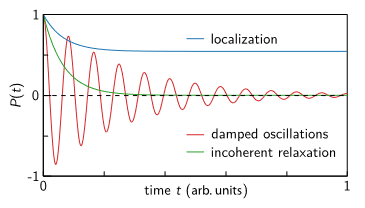
\includegraphics[width=\columnwidth]{20230813.png}}
    \caption{}
    \label{figure_1} 
\end{figure}
\end{document}
